\section{Phase 3: High Fidelity Prototype}

\subsection{Methodology}
We used the 
responses % JRB: Word choice? Maybe "Insights", because you analyzed the results, right? :D
from the low fidelity prototype study to design a fully immersive StoAR prototype for use in head-mounted displays. Because we did not have access to a retail testing environment, we simulated a retail display in virtual reality based on configurations found in a local retail outlet. We then added an augmented reality interface to the simulation to provide review and price information, depicted in Figure 2.\todo{briefly describe the important pieces informed by the low-fi study} \todo{Add figure according to CHI LBW format} While our use of a VR store simulation removes immediate access to real life product found in a real world store, the fully immersive environment allowed us to closely control the relationship between the prototype AR interfaces and simulated products. %and reduced the environmental complexity to allow participants to focus solely on the prototype implementation. 

\begin{figure}
	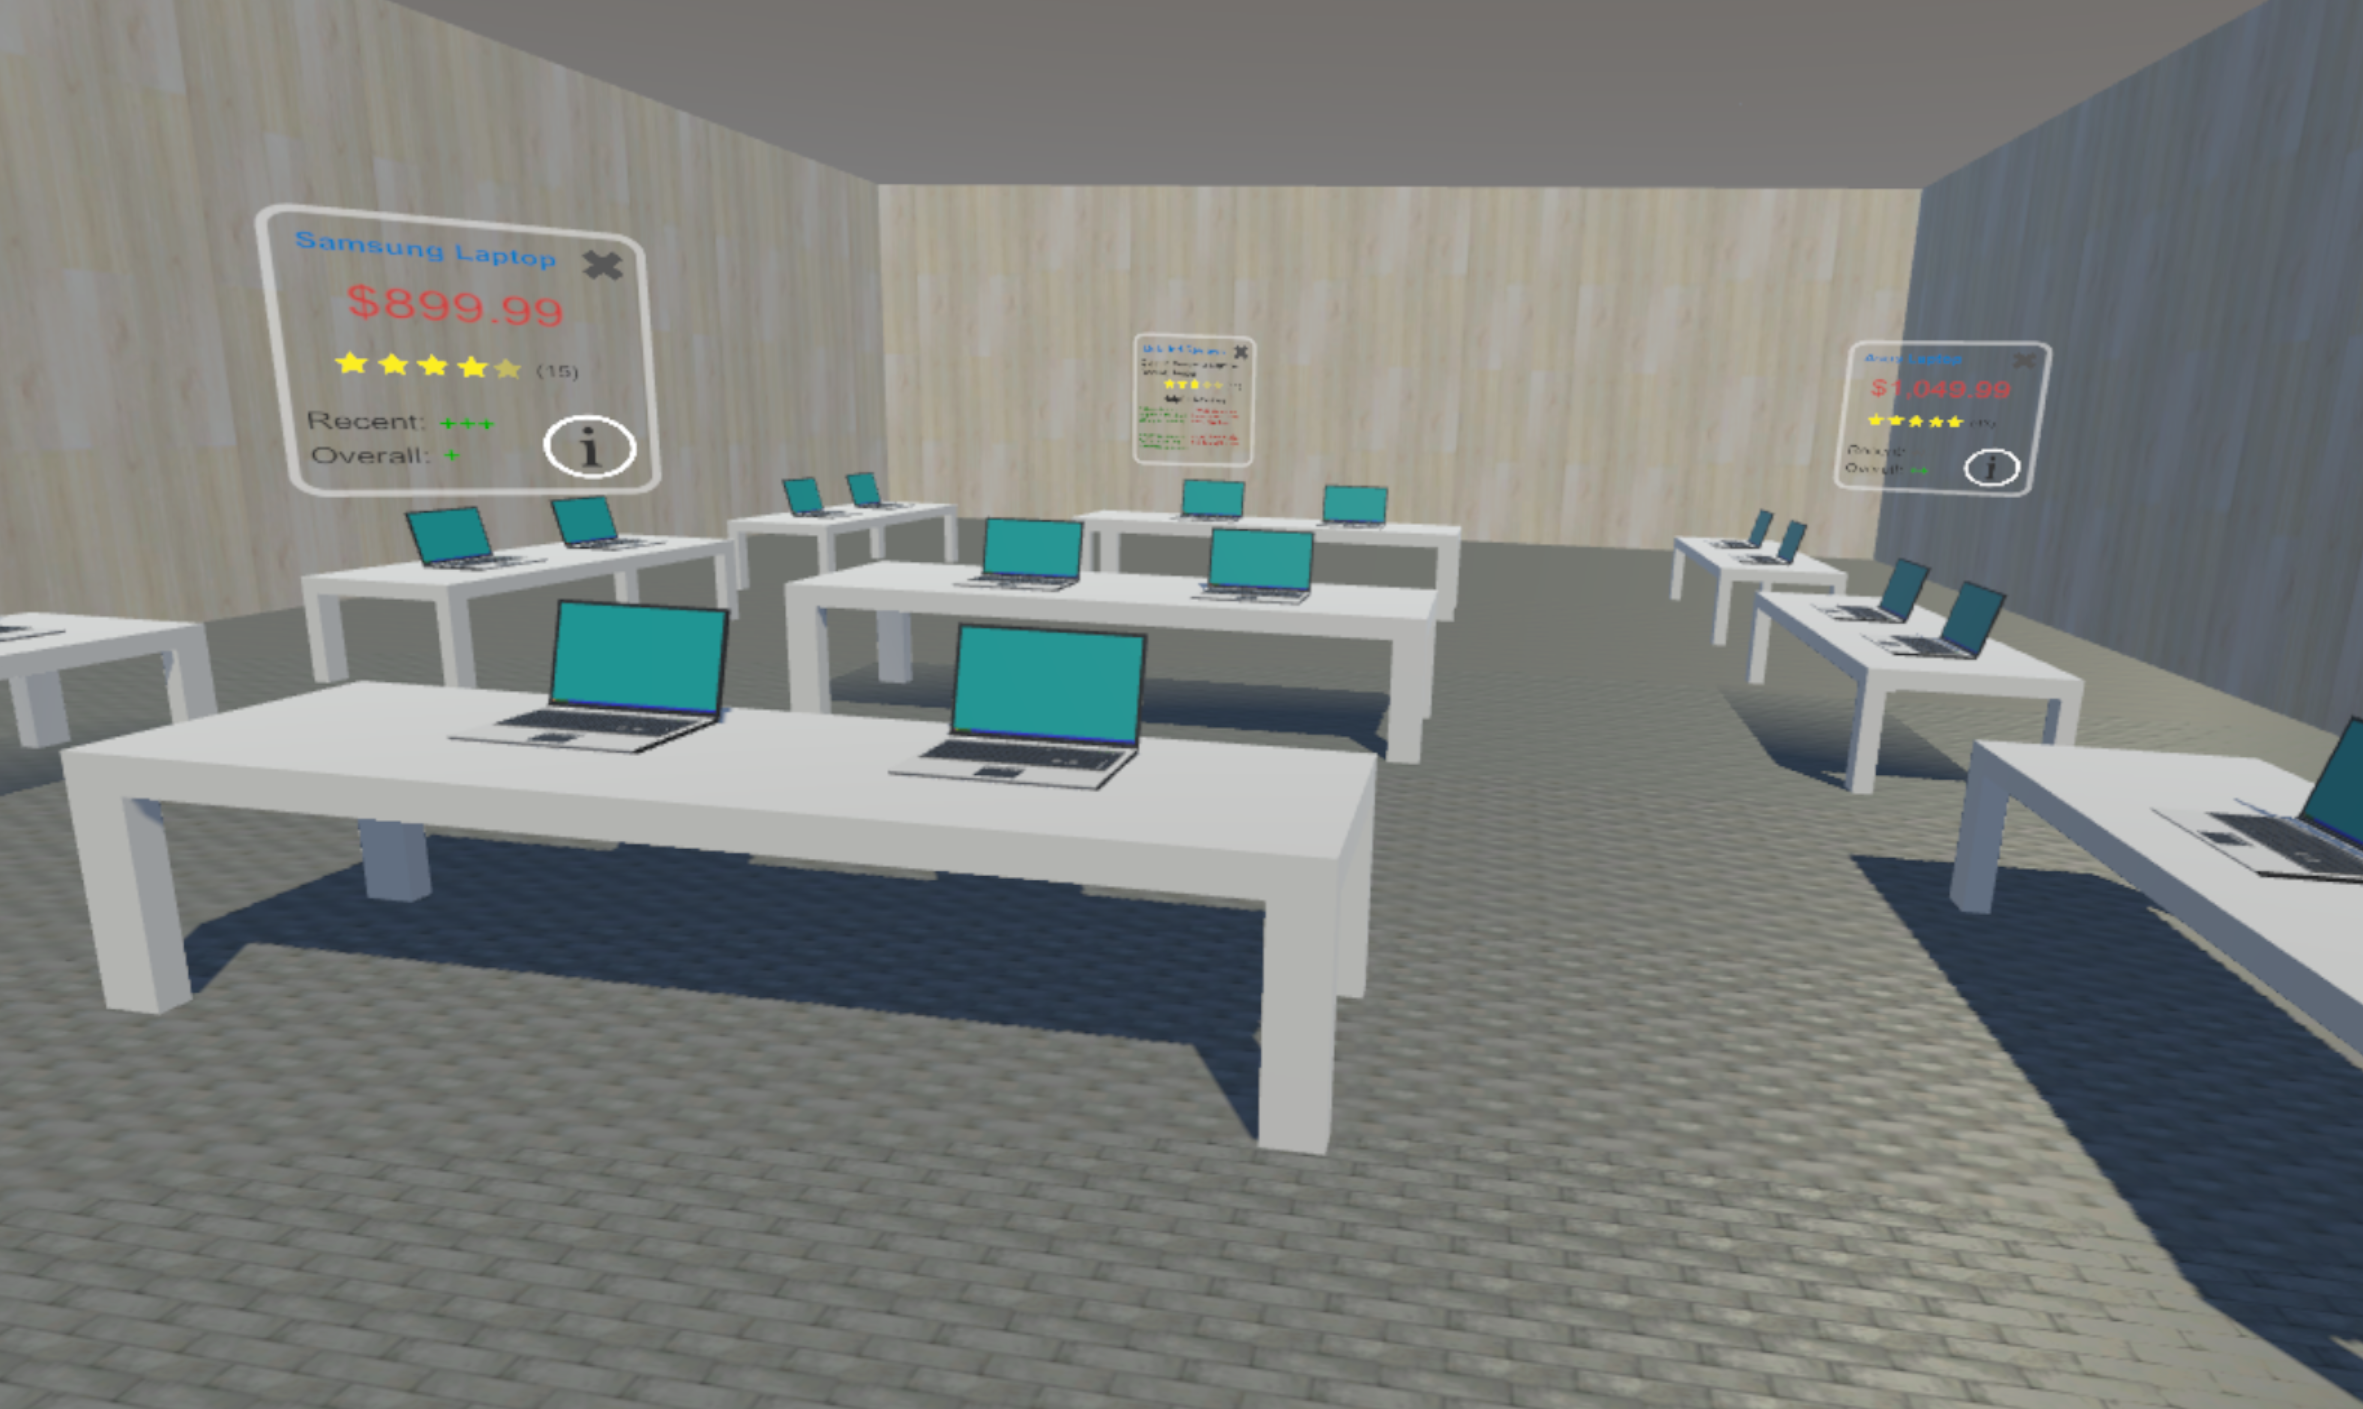
\includegraphics[width=0.9\columnwidth]{figures/3Panel}
	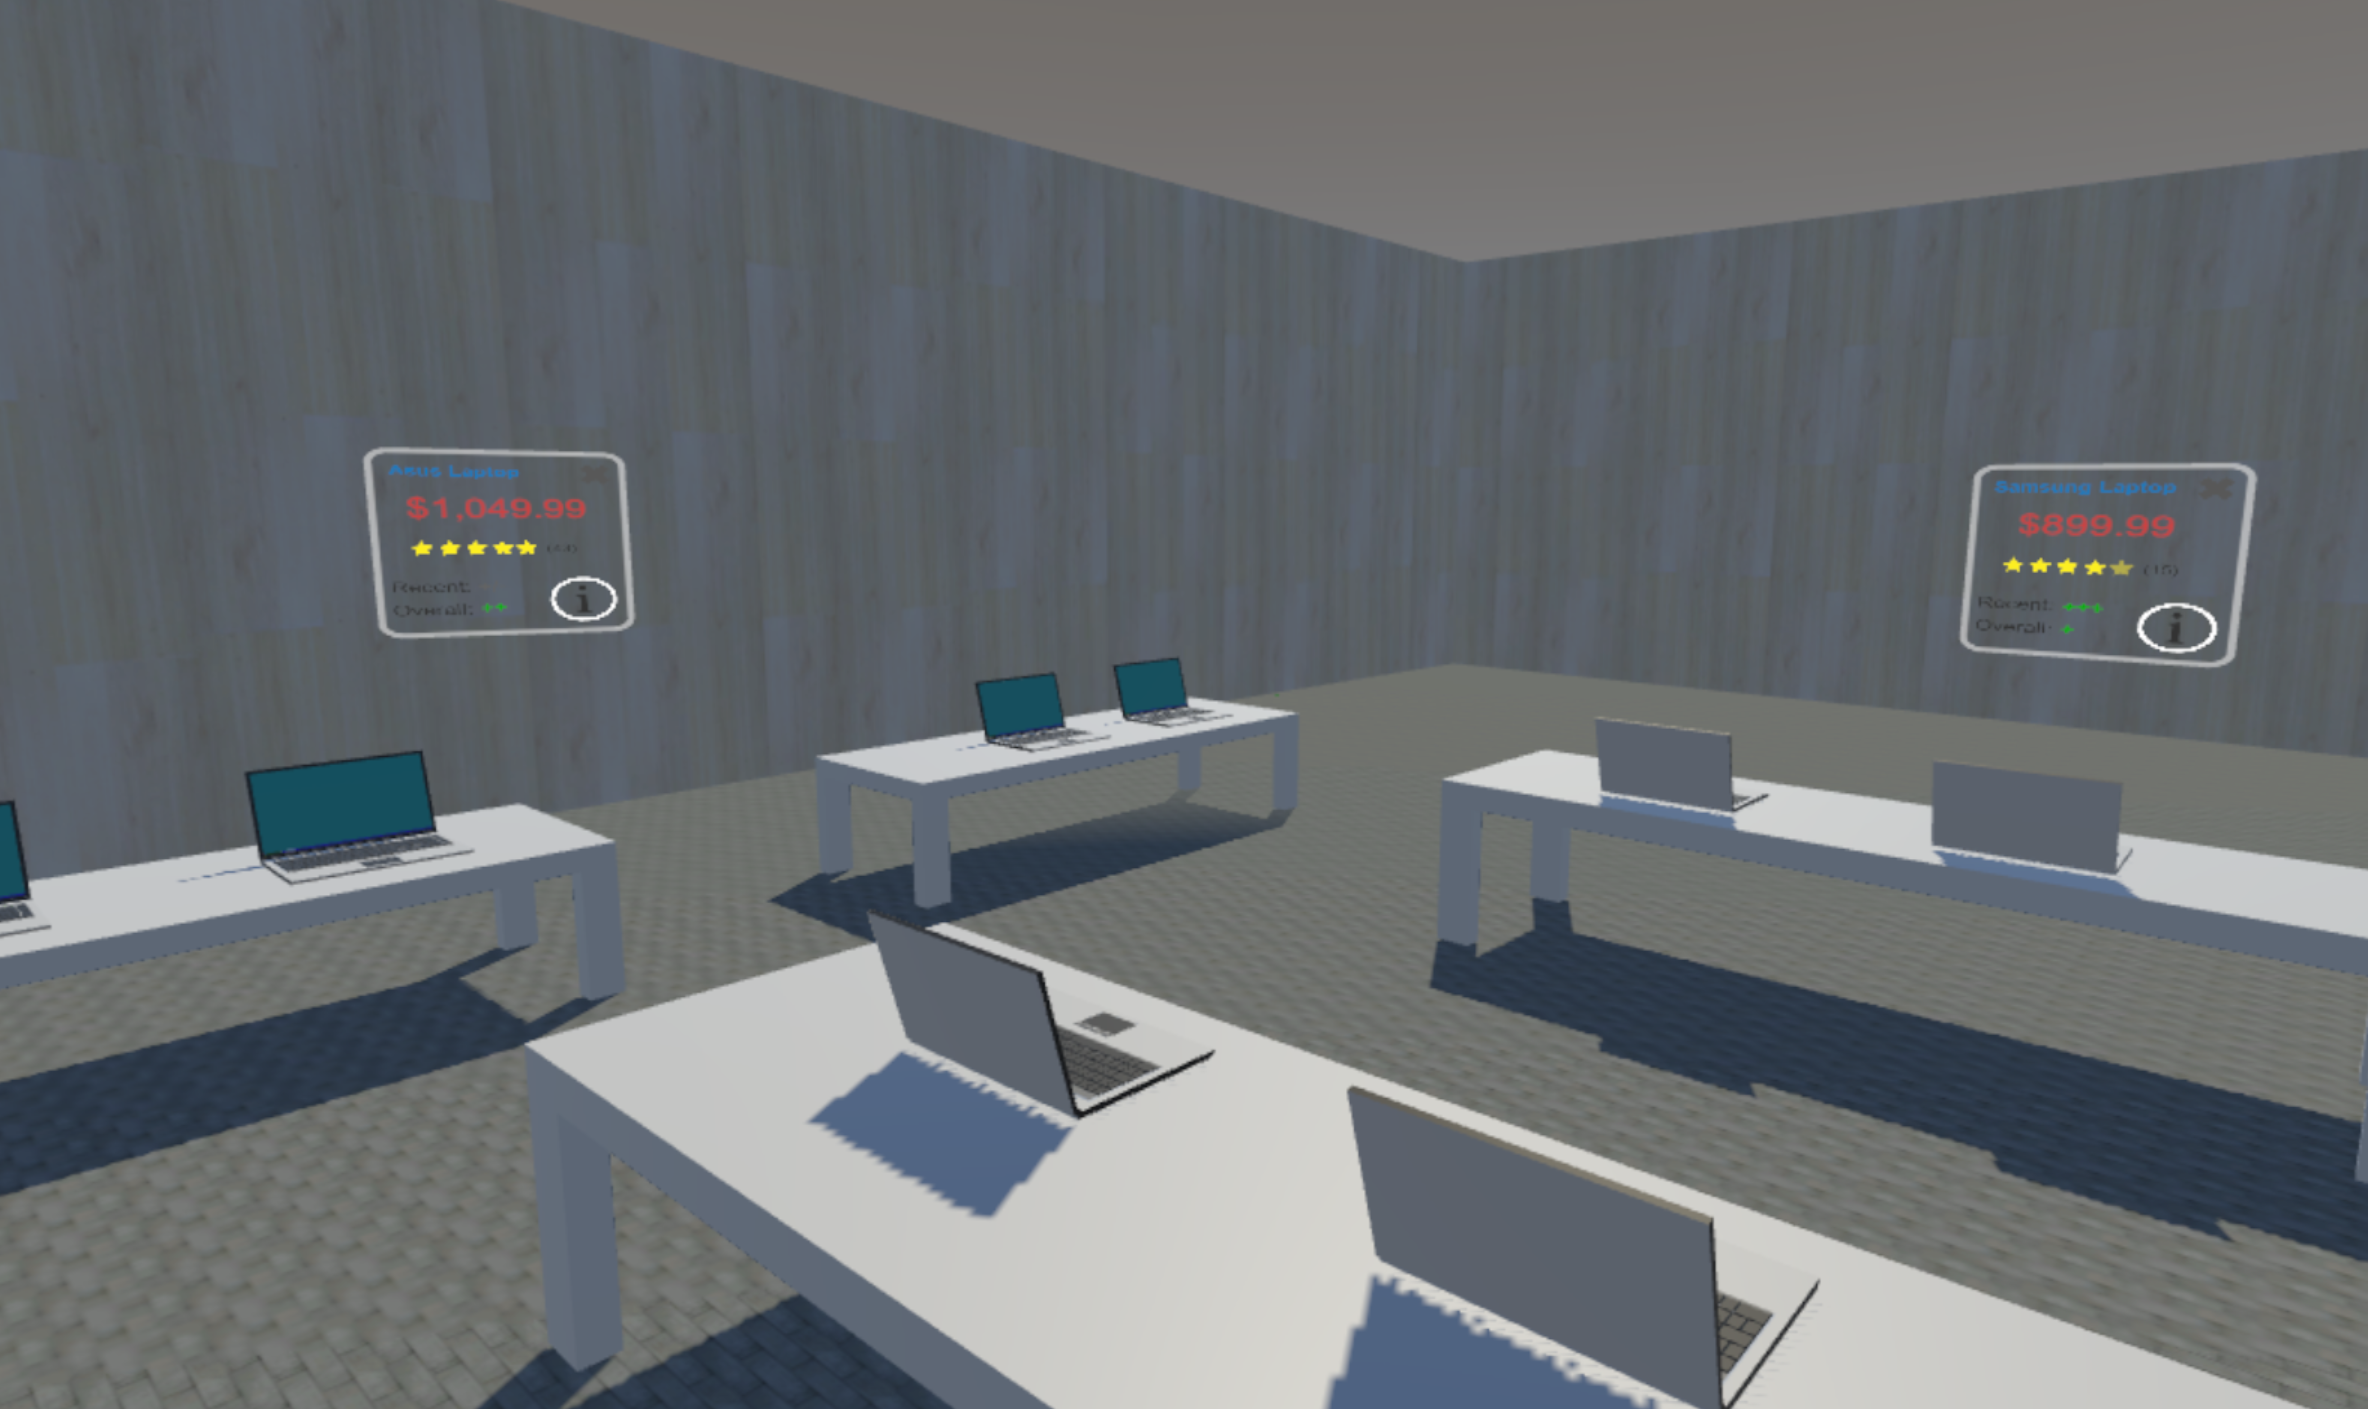
\includegraphics[width=0.9\columnwidth]{figures/2Panel}
	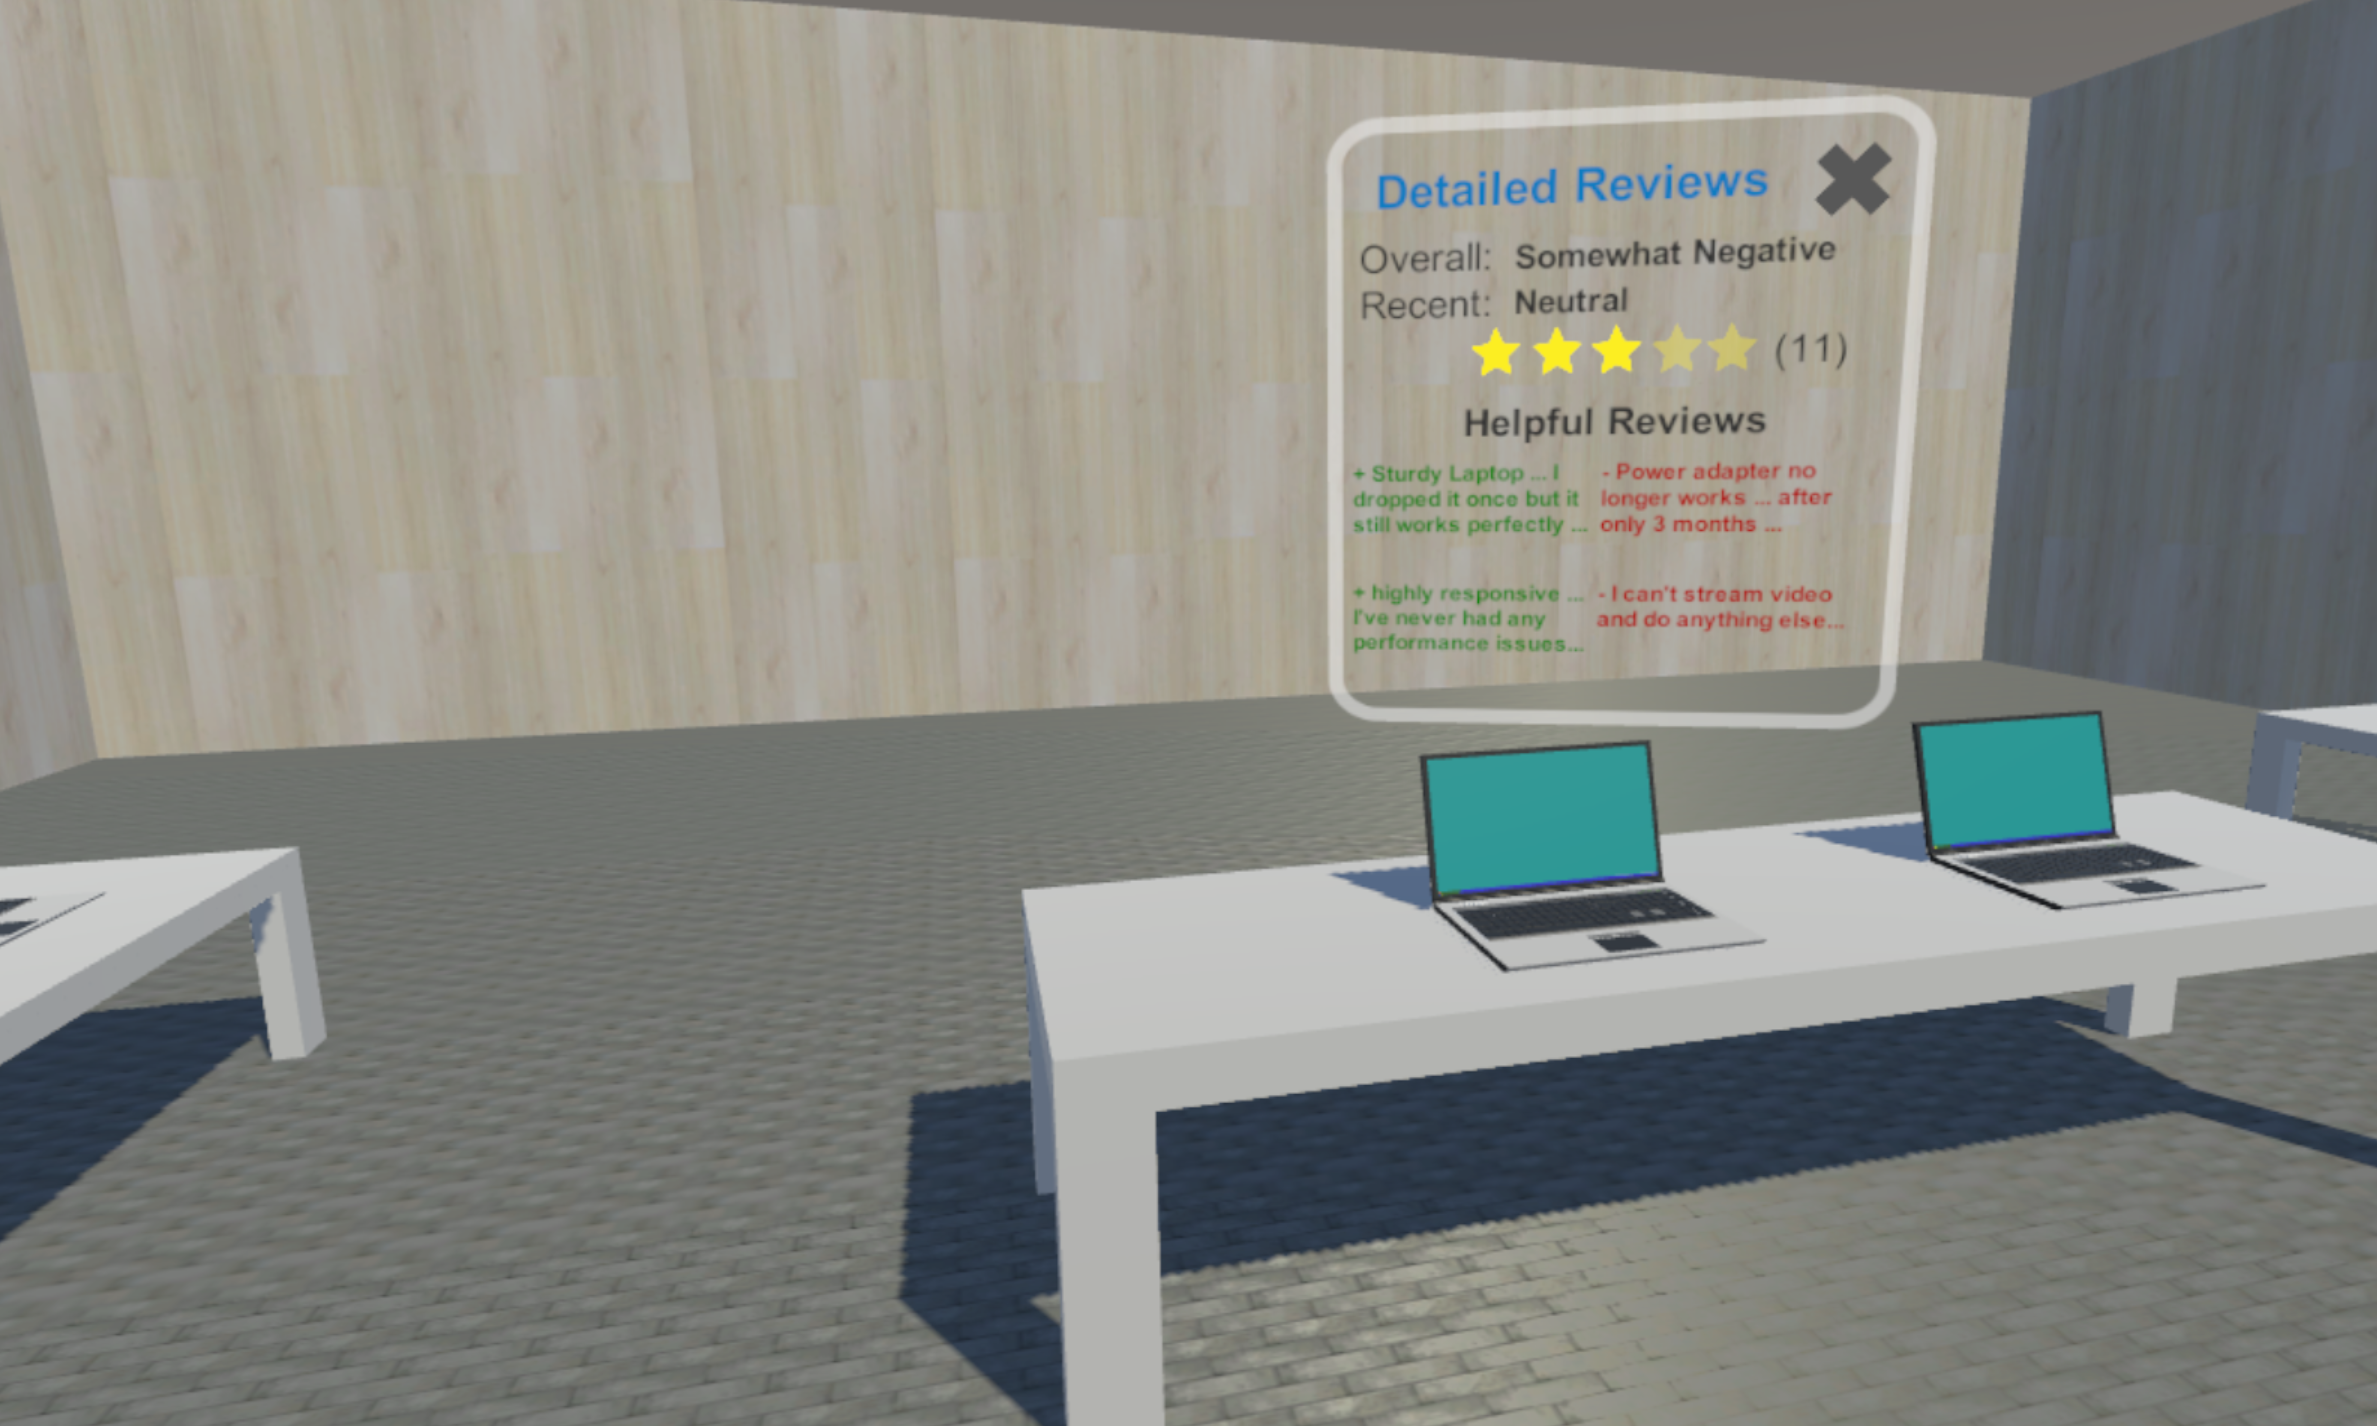
\includegraphics[width=0.9\columnwidth]{figures/DetailReviews}
	\caption{Screenshots of high fidelity protoype VR experience}
	\label{figures:HiFiScreenshots}
\end{figure}

We recruited 20 participants from a local research expo to use our prototype and provide feedback. Participants first freely navigated the virtual representation of a store augmented with static content containing information about each device.
%Given space constraints, the track pad on one of the Vive's controllers was employed for users to navigate within the scene.
After navigating the scene, participants completed a short survey that asked for their perceptions of the prototype's usability, potential impact on decision-making, utility of individual design components, perceived trade-offs compared to existing technologies and potential limitations of the approach. They also provided feedback on additional applications where they envisioned using mixed reality experiences for decision making. As with the initial online survey, we analyzed the qualitative feedback provided by users by clustering their responses into common themes.
%The survey asked for specific product-domains to which our system could be applied (i.e. electronics, furniture, books).  

Participants said they envision using this platform for comparison shopping, quickly seeing reviews, prices, and product specifications, and visual demonstrations of product use. 
Lower depth of product information was provided as a trade-off of the system. % JRB: Clarification please.
Participants expressed concern about digital content distracting them from the physical environment. Having presented them with laptops, we asked participants for what other products they 
think % JRB: w/c? Thought?
augmented reality could aid them in decision-making, with the results shown in figure \ref{figures:HiFiScreenshots}. \todo{MW: Games, toys, furniture, and clothing.  Honestly, this finding doesn't really line up with anything else, unless we start drawing conclusions about "They said furniture because of potential for visualizations" or something like that. We have a figure if we want to keep this point.} 

We prompted participants for additional features of a retail augmented reality system such as this one. Participants detailed several expected interactions with the static content provided. Aligning with feedback from the low-fidelity prototypes, participants wanted to keep information within a single view such that they could comparison shop. With the way content was provided in the high-fidelity prototype, users would need to turn around or walk toward another laptop to view its associated information. Participants expressed that they want to compare prices of the same product against other stores' prices. If presented with the option, participants said they would consider purchasing from another source. \todo{JRB: Same comment as Phase 2. This is a list of what they told you. Can you take it one step further and tell us what this means? What are the implications of these comments? You said you did this -- "We explored how understanding the trade-offs of parallel physical and virtual experiences could inform mixed reality applications in the context of retail shopping." -- so tell me what the results of this phase told you about those trade-offs. }